\section{Propriedades dos sistemas de recomendação}
\subsection{\textit{Feedback} explícito vs. implícito}

Em geral, recomendações personalizadas são baseadas no \textit{feedback} dos
usuários, ou seja, em informações providas pelos usuários, utilizadas para
identificar suas preferências. Essas informações são ações explícitas ou dados
inferidos de forma implícita.

Historicamente, a pesquisa inicial de sistemas de recomendação foi dominada por
cenários nos quais os usuários declaram explicitamente seu interesse em itens,
principalmente na forma de avaliações de itens em uma escala numérica de 1 a 5.
Esses algoritmos modelam o problema como uma tarefa de preenchimento da matriz
de avaliações.

A facilidade de obter \textit{feedbacks} explícitos preenchidos por usuários
depende do domínio da aplicação. Por exemplo, em sistemas de consumo de
produtos, como comércio eletrônico ou \textit{streamings} de mídia. Por outro
lado, uma aplicação sem qualquer forma de avaliação explícita torna o sistema de
recomendação dependente de informações comportamentais monitoradas dos usuários,
ou seja, de \textit{feedback} implícito \cite{ludewig2020advances}.

O \textit{feedback} implícito do usuário é caracterizado por ações diretamente
observáveis do usuário ou sinais de preferência indiretos, relacionados a
características ou ações do
usuário.

A dificuldade na diferenciação de um sinal como interesse ou desinteresse é uma
das desvantagens do \textit{feedback} implícito. Por exemplo, quando um usuário
assiste a um vídeo curto em uma interface de \textit{Feed} como o TikTok ou
Instagram, o usuário assistir o vídeo por completo não é necessariamente
modelado como um \textit{feedback} positivo. Por sua vez, o usuário descartar
imediatamente determinado vídeo pode ser interpretado como \textit{feedback}
negativo. Apesar disso, sistemas de \textit{feedback} implícito em geral não contam
com sinais negativos \cite{ludewig2020advances,JLZ18}.

\subsection{Sistemas de recomendação baseados em contexto} Abordagens
tradicionais de sistemas de recomendação ignoram a ordem e o contexto do
\textit{feedback} do usuário. Por exemplo, uma mudança nas preferências de longo
e curto prazo do usuário, a sazonalidade de um produto, um interesse pontual ou
o reinteresse em um item já consumido. A detecção e distinção dessas
preferências influenciam positivamente na assertividade das recomendações.

Padrões semelhantes são encontrados em diferentes aplicações. Nomes específicos
foram cunhados para distingui-los, como a recomendação \textit{context-aware},
\textit{time-aware} e \textit{sequence-aware}. Essas áreas compartilham
características e similaridades. Por exemplo, sistemas \textit{session-based}
são considerados um caso particular de sistemas \textit{context-aware}, em que o
contexto é simplificado e delimitado por uma sessão \cite{survey_wang_2021}.
Sistemas \textit{time-aware} são considerados um caso particular de sistemas
\textit{sequence-aware}, em que o instante de tempo de cada interação é
registrado e capaz de modelar a sequência de interações
\cite{ludewig2020advances}.

\subsubsection{\textit{Context-aware}} 

Em sistemas de recomendação tradicionais, a estimativa da utilidade de um item a
um determinado usuário é obtida em função desses dois dados. Dessa forma,
usuário e item são as duas entidades fundamentais nesses sistemas. Apesar disso,
uma série de outros fatores podem influenciar nas preferências do usuário. Por
exemplo, o dia no ano, a localização e o clima podem impactar as preferências de
compra de itens típicos associados a praias ou a invernos rigorosos. Essas
informações são consideradas fatores contextuais \cite{rec_sys_handbook_2022_context}.
Sistemas \textit{context-aware} estimam a utilidade de um item em função de três
entidades: usuário, item e contexto.

A disponibilidade dos fatores contextuais é classificada como explícita ou
latente. Contextos explícitos são informações diretamente observáveis e
mensuráveis. Contextos latentes são aqueles que não podem ser medidos
diretamente, mas podem ser inferidos a partir de modelos de fatores latentes ou
de \textit{embeddings} em modelos de aprendizado profundo.

Por sua vez, a mutabilidade dos fatores contextuais ao longo do tempo é
classificada como estática ou dinâmica. Contextos estáticos são informações com
associação e valor inalterados ao longo do tempo. Por exemplo, informações
contextuais de instante e preço de compra em um comércio eletrônico permanecem
inalterados. Contextos dinâmicos são informações que podem ser alteradas ao
longo do tempo. Por exemplo, informações de contexto do usuário vigente, no
instante em que uma recomendação é realizada
\cite{rec_sys_handbook_2022_context}.

\subsubsection{\textit{Time-aware}}

A informação da data da interação destaca-se
pela facilidade de obtê-la explicitamente, uma vez que a grande maioria dos
sistemas registram o instante de tempo associado às avaliações ou ao consumo de
determinado item. Sistemas de recomendação \textit{time-aware} são um caso
particular de sistemas \textit{context-aware}, em que o contexto é delimitado
pela dimensão temporal.

Geralmente, sistemas \textit{time-aware} utilizam o instante de tempo da
interação, porém outras fontes de informação temporal, como a data de
incorporação de um item no catálogo do sistema ou a data de registro do usuário,
tornam o sistema em questão \textit{time-aware}.

Por mais que sistemas \textit{time-aware} sejam capazes de inferir preferências
de curto e longo prazo, a dependência de informações temporais torna-os
suscetíveis a problemas de \textit{cold-start} \cite{rec_sys_handbook_2022_multi}.

\subsubsection{\textit{Sequence-aware}}
A recomendação \textit{sequence-aware} é dedicada a sequências e padrões
repetitivos no \textit{feedback} dos usuários. Sistemas \textit{session-aware} e
\textit{session-based} são classificados como uma subárea da recomendação
\textit{sequence-aware}.

Em geral, os dados de entrada em um problema \textit{sequence-aware} são listas
de interações do usuário em ordem cronológica. Nos casos em que consta o instante
de tempo de cada interação, também trata-se de um problema \textit{time-aware}.

Sistemas \textit{sequence-aware} são modelados a partir de sequências ordenadas
de interações, sem necessariamente delimitar as ações em sessões. Não há
modelagem explicita agrupando conjuntos de interações. As preferências de longo
ou curto prazo são inferidas a partir da ordem, da co-ocorrência ou da distância
entre interações \cite{sessionbaseddp, quadrana2018sequence}.


\section{Sistemas de Recomendação aplicados ao Indaband}

\subsection{Sistemas de Recomendação \textit{Session-Based} e \textit{Session-Aware}}

Os SBRS são aplicáveis quando os dados
 de entrada do modelo consistem em um conjunto ou uma sequência de interações do usuário
 durante uma mesma sessão de itens, tal que \cite{survey_wang_2021}:

 \begin{equation*}
  \begin{aligned}
  U & = \{u_1, u_2, \ldots, u_{|U|}\} \\
  V & = \{v_1, v_2, \ldots, v_{|V|}\}
\end{aligned}
\end{equation*}

$U$ é o conjunto de todos os usuários existentes. O usuário $u$ equivale ao
usuário que executa uma ação, como a criação de uma sessão. $V$ é o conjunto de
todos os $v$ itens existentes.

\begin{equation*}
  \begin{aligned}
  A & = \{a_1, a_2, \ldots, a_{|A|}\} \\
  o & = <v, a> \\
  O & = \{o_1, o_2, \ldots, o_{|O|}\}
  \end{aligned}
  \end{equation*}
$A$ é o conjunto das ações, tais como: criação de sessão, convite endereçado a
  determinado usuário, gravação, etc. Cada $o$ interação é a tupla entre item e
  ação, enquanto que $O$ é o conjunto de todas as interações.

  A principal distinção entre SBRS e sistemas de recomendação \textit{session-aware}
  é a ausência de identificação do usuário que realiza as ações sobre os itens.
  Ou seja, no caso \textit{session-aware}:

  \begin{equation}
    o = <u, v, a>
    \end{equation}
  em que a interação é uma tupla entre usuário, item e ação.

  \begin{equation*}
  \begin{aligned}
  s & = [o_1, o_2, \ldots, o_{|s|}] \\
  S & = \{s_1, s_2, \ldots, s_{|S|}\} \\
  \hat{l} & = [\hat{o}_1, \hat{o}_2, \ldots, \hat{o}_{|\hat{l}|}]
  \end{aligned}
  \end{equation*}
  
    Por sua vez, a sessão $s$ é uma lista de $|s|$ interações, tal que o
  conjunto de todas as sessões é dado por $S$. A lista de $\hat{o}$ interações
  recomendadas é dada por $\hat{l}$.

  O objetivo de um SBRS é selecionar uma lista recomendada de interações
  que maximize a função de desempenho $f(s, c)$ condicionada ao contexto $c$ da
  sessão $s$:
  \[\hat{l} = \arg \max f(s, c), \quad c \in C, \quad s \in S.\]   

 O contexto $c$ é definido como um conjunto de informações adicionais associadas
  à sessão e que podem ser utilizadas para melhorar a assertividade das
  recomendações.  Hora do dia, clima e localização do usuário são parâmetros os
  quais podem ser incluídos por contexto.

  É importante destacar que $s$ e $S$ podem
  ser definidos com um conjunto de interações desprovido de ordenação temporal
  ou como listas ordenadas de interações e de sessões. Essas duas abordagens
  dependem das propriedades \textit{context-aware}, \textit{time-aware}
  e \textit{sequence-aware} do sistema de recomendação.

  No caso das recomendações \textit{session-based} e \textit{session-aware},
  cada interação é associada a um identificador de sessão, agrupando várias
  interações consecutivas. As interações são agrupadas em uma única sessão até
  que o usuário não execute nenhuma interação por um período específico de
  tempo, geralmente após trinta minutos de ociosidade.
  
  Ao contrário da recomendação \textit{sequence-aware}, os recomendadores
  \textit{session-aware} necessariamente consideram a sessão atual do usuário.
  Na recomendação \textit{sequence-aware}, algumas técnicas dependem apenas do
  histórico de longo prazo dos usuários, levando em consideração a ordem dos
  eventos.

  No caso do presente trabalho, em que deseja-se
recomendar usuários a serem convidados, os conjuntos $U$ e $V$ são iguais nessa
aplicação específica:
\begin{equation*}
\begin{aligned}
  U & = V \\
  u_n & = v_n
\end{aligned}
\end{equation*}

  % \subsection{Características}


% A recomendação \textit{session-based} pode ser interpretada tanto como
% \textit{sequence-aware} quanto \textit{session-aware} em cenários de
% \textit{cold-start} do usuário, ou seja, na ausência de informações históricas
% para todos os usuários. Por outro lado, a recomendação \textit{session-based} é
% desprovida de modelos personalizados de longo prazo. A personalização das
% sugestões de itens depende exclusivamente das últimas interações do usuário.

  \subsection{Avaliação de desempenho em SBRS} \label{chap:desempenho}
  A ideia geral da avaliação em SBRS consiste em revelar uma parte das interações
  iniciais de uma sessão e comparar as interações recomendadas subsequentes com
  as interações que o usuário realmente realizou.
  
  Três abordagens são utilizadas na literatura para avaliar o desempenho de
  sistemas \textit{session-based} e \textit{session-aware}: \textit{next-item},
  \textit{remaining items} e \textit{last-item}.

  Na abordagem \textit{next-item}, as primeiras $N$ interações de uma sessão de
  teste são reveladas ao sistema de recomendação e apenas a interação
  subsequente é utilizada como prova real e comparada com o valor recomendado.
  Dessa forma, o sistema pode revelar item a item e avaliar cada recomendação,
  ou revelar apenas o último item de cada sessão.

  Por sua vez, a abordagem \textit{remaining items} revela todos os itens
  subsequentes ao realizar a prova real. O valor recomendado é comparado
  com todos os itens subsequentes, e não apenas com o próximo item.

  A abordagem \textit{last-item} avalia diretamente o último item de cada
  sessão. Essa abordagem não aproveita as interações intermediárias para
  avaliação, focando apenas no último item da sequência.

  \abbrev{HR}{\textit{Hit Rate}} \abbrev{MAP}{\textit{Mean Average Precision}}
  \abbrev{MAR}{\textit{Mean Average Rank}} \abbrev{NDCG}{\textit{Normalized
  Discounted Cumulative Gain}} Para as abordagens \textit{next-item} e
  \textit{last-item}, as métricas de avaliação utilizadas são \textit{Hit Rate}
  (HR) e \textit{Mean Reciprocal Rank} (MRR). Para a abordagem \textit{remaining
  items}, as métricas de avaliação utilizadas são a Precisão, \textit{Recall},
  \textit{Mean Average Precision} (MAP), \textit{Mean Average Rank} (MAR),
  \textit{Normalized Discounted Cumulative Gain} (NDCG) e \textit{F1}
  \cite{sessionbaseddp}.

  Uma vez que sistemas de recomendação tendem a enviesar as recomendações para
  itens populares, as métricas de cobertura e popularidade são utilizadas para
  avaliar a diversidade e o viés das recomendações. Sessões assertivas com pouco
  viés de popularidade e maior cobertura indicam maior qualidade na
  personalização das recomendações.

  \subsubsection{\textit{Hit Rate} (HR)}
  O HR@N é a porcentagem de vezes em que um item relevante
  é recomendado entre os $N$ primeiros itens da lista de recomendações~\cite{sessionbaseddp}:

  \begin{equation}
    % \text{HR}_{\text{N}} = \frac{1}{|U|} \sum_{u \in U} \sum_{i \in R_{u, N}} \frac{1}{N}
    \text{HR@N} = \frac{1}{Q}\sum_{i=1}^{Q}\begin{cases}
      1 & \text{se} \quad i \leq N \\
      0 & \text{caso contrário}
    \end{cases}
  \end{equation}
  em que $Q$ é o comprimento da lista de itens recomendados para uma determinada
  predição e $i$ é a posição do item na lista de recomendações.
  \subsubsection{\textit{Mean Reciprocal Rank} (MRR)} O MRR@N é similar ao HR@N,
  porém leva em consideração a posição do item. Se o item recomendado
  corretamente consta nas primeiras posições da lista de recomendações, o MRR@N
  é maior, decaindo conforme a posição do item recomendado corretamente fica
  mais distante do início da lista de recomendações. Por sua vez, o incremento
  no HR@N em razão de um item recomendado no início ou no final da lista contém
  pesos idênticos~\cite{sessionbaseddp}.

  \begin{equation}
    \text{MRR@N} = \frac{1}{Q}\sum_{i=1}^{Q}\begin{cases}
      \dfrac{1}{i} & \text{se} \quad i \leq N \\
      0 & \text{caso contrário}
    \end{cases}
  \end{equation}

  \subsubsection{Precisão e \textit{Recall}}
  No contexto de classificadores, a precisão e o \textit{recall} avaliam
  a qualidade de um modelo a partir da matriz de confusão descrita
  na tabela \ref{tab:confusion_matrix}::

  \begin{align}
    \text{Precisão} &= \frac{\text{VP}}{\text{VP} + \text{FP}} \\
    \text{\textit{Recall}} &= \frac{\text{VP}}{\text{VP} + \text{FN}}
  \end{align}

  \begin{table}[H]
    \centering
    \begin{tabular}{c|c|c|}
      \cline{2-3}
      & \multicolumn{2}{c|}{\textbf{Predição}} \\ \cline{2-3} 
      & \textbf{Positivo} & \textbf{Negativo} \\ \hline
      \multicolumn{1}{|c|}{\textbf{Positivo}} & Verdadeiro Positivo (VP) & Falso Positivo (FP) \\ \hline
      \multicolumn{1}{|c|}{\textbf{Negativo}} & Falso Negativo (FN) & Verdadeiro Negativo (VN) \\ \hline
    \end{tabular}
    \caption{Matriz de confusão}
    \label{tab:confusion_matrix}
  \end{table}
  \abbrev{VP}{Verdadeiro Positivo}
  \abbrev{FP}{Falso Positivo}
  \abbrev{FN}{Falso Negativo}
  \abbrev{VN}{Verdadeiro Negativo}

  No contexto de sistemas de recomendação, a Precisão@N avalia a quantidade de
  itens relevantes em relação ao total de $N$ itens recomendados na lista~\cite{sessionbaseddp}. O conjunto
  dos $N$ itens recomendados equivale aos verdadeiros e falsos positivos:

  \begin{equation}
    \text{Precisão@N} = \frac{\text{Qntd. de itens relevantes nas primeiras N recomendações}}{N}
  \end{equation}

  Por sua vez, o Recall@N equivale a quantidade de itens relevantes entre
  os $N$ primeiros itens da lista de recomendações, desconsiderando a
  posição do item na lista. O conjunto dos itens relevantes equivale
  aos verdadeiros positivos e falsos negativos:

  \begin{equation}
    \text{Recall@N} = \frac{\text{Qntd. de itens relevantes nas primeiras N recomendações}}{\text{Quantidade de itens relevantes}}
  \end{equation}

  \subsubsection{\textit{Mean Average Precision} (MAP)} O MAP@N calcula a média
  da precisão média (AP@N) para cada consulta. Após cada item relevante ser
  recomendado, a precisão é medida, tal que a média é calculada por~\cite{carnevali2023offline}:

  \begin{align}
    \text{AP@N} &= \frac{\sum_{i = 1}^{K}\text{Precisão@k} \times \text{rel}_{k}}{\text{qntd. de resultados relevantes}} \\
    \text{rel}_k &= \begin{cases}
      1 & \text{se} \quad k \leq N \\
      0 & \text{caso contrário} 
    \end{cases} \\
    \text{MAP@N} &= \frac{1}{Q}\sum_{q = 1}^{Q} \text{AP@N}_{q}
  \end{align}
  em que $K$ é a quantidade de itens recomendados, $\text{rel}_{k}$ é a
  relevância do item na posição $k$ e $Q$ é a quantidade de consultas.

  \subsubsection{\textit{Normalized Discounted Cumulative Gain} (NDCG)}
  O NDCG é baseado no ganho cumulativo (CG). O ganho cumulativo é a soma dos
  valores de relevância graduais de todos os itens em uma lista de
  recomendações~\cite{carnevali2023offline}:

  \begin{equation}
    \text{CG@N} = \sum_{i = 1}^{N} \text{rel}_{i}
  \end{equation}
  
  \abbrev{CG}{\textit{Cumulative Gain}}
  \abbrev{DCG}{\textit{Discounted Cumulative Gain}}
  \abbrev{IDCG}{\textit{Ideal Discounted Cumulative Gain}}
  Por sua vez, o NDCG é a razão entre o ganho cumulativo
  descontado (DCG) e o ganho cumulativo descontado ideal (IDCG). Ambos contém
  um fator de penalidade no denominador:

  \begin{align}
    \text{DCG@N} &= \sum_{i = 1}^{N} \frac{2^{\text{rel}_{i}} - 1}{\log_{2}(i + 1)} \\
    \text{IDCG@N} &= \sum_{i = 1}^{\text{REL}_N} \frac{\text{rel}_{i}}{{\log_{2}(i + 1)}} \\
    \text{NDCG@N} &= \frac{\text{DCG@N}}{\text{IDCG@N}}
  \end{align}
  em que $\text{REL}_N$ é a lista de itens relevantes contidos em $N$, ordenados
  por relevância.


  \subsubsection{F1}
É calculado a partir da média harmônica entre a precisão e o \textit{recall}. Dessa forma,
um valor baixo ou próximo de zero para qualquer uma dessas duas métricas derruba
o valor do F1~\cite{sessionbaseddp}:

\begin{equation}
  \text{F1} = \frac{2 \times \text{Precisão} \times \text{Recall}}{\text{Precisão} + \text{Recall}}
\end{equation}

  \subsubsection{Cobertura}
  A cobertura mede a proporção de itens recomendados em relação ao total de
  itens disponíveis. Se definirmos o conjunto de itens disponíveis como $I$ e o
  conjunto de itens recomendados como $I_{p}$, a cobertura é dada por~\cite{sessionbaseddp}:
  \begin{equation}
    \text{Cobertura@N} = \frac{|I_{p}|}{|I|}.
  \end{equation}


\abbrev{RNN}{redes neurais recorrentes}
\subsection{RNN}
Redes neurais recorrentes (RNNs, do inglês \textit{recurrent neural networks})
 são apropriadas para dados que tenham uma relação de sequência entre si
 \cite{gru4rec_1}. Sua principal diferença em relação aos demais modelos de
 aprendizado profundo é a existência de um estado oculto $\mathbf{h_t}$ em
 cada unidade da rede, cujo valor é obtido a partir da seguinte função de
 atualização:
 \symbl{$\mathbf{h_t}$}{estado oculto da unidade no instante $t$}
\begin{equation}
    \mathbf{h_t} = g(W\mathbf{x_t} + U\mathbf{h_{t-1}})
\end{equation}
onde $g$ é uma função suave e limitada entre 0 e 1, como uma função logística
sigmoide ou tangente hiperbólica, $\mathbf{x_t}$ é a entrada da unidade no
instante atual, $W$ e $U$ são os pesos associados à entrada e ao estado
anterior, $\mathbf{h_{t-1}}$ é o estado no instante anterior. Uma RNN gera uma
distribuição de probabilidade sobre o próximo elemento da sequência a partir do
estado atual:

\begin{equation}
    p(\mathbf{x_t}|\mathbf{x_1},\ldots , \mathbf{x_{t-1}}) = g(\mathbf{h_t})
\end{equation}

Um problema típico da arquitetura básica de RNNs é o desaparecimento ou explosão
do gradiente ao minimizar a função de custo, uma vez que o incremento ou
decremento do gradiente equivale ao produtório dos pesos de todas as unidades, o
que converge para um valor minúsculo ou diverge para um valor enorme. Unidades
sob a forma de LSTMs ou GRUs foram propostas para resolver esse problema.


\subsection{LSTM}
\abbrev{LSTM}{memória de curto e longo prazo}
A memória de curto e longo prazo (LSTM, do inglês \textit{long short-term
memory}) \cite{chung2014empirical} substitui a unidade típica de uma RNN. Sua
principal melhoria, tanto na LSTM é a capacidade de manter o estado atual
de suas células, em vez de sobrescrevê-lo a cada iteração. Dessa forma, a
unidade pode detectar e manter informações relevantes de forma dinâmica,
inclusive em sequências longas.

Sua arquitetura resolve os problemas de dissipação ou explosão do
gradiente, uma vez que a etapa de \textit{backpropagation} não envolve a
multiplicação de todos os pesos.

A LSTM é composta por uma célula de memória $\mathbf{c_t}$. A saída, ou ativação
$\mathbf{h_t}$, é dada por:
\begin{equation}
    \mathbf{h_t} = \mathbf{o_t}\tanh(\mathbf{c_t})
\end{equation}
em que $\mathbf{o_t}$ é a porta de saída, a qual controla a quantidade de
exposição, cujo valor é dado por:

\begin{equation}
    \mathbf{o_t} = \sigma(W_o\mathbf{x_t} + U_o\mathbf{h_{t-1}} + V_o\mathbf{c_t})
\end{equation}
em que $\sigma$ é a função logística sigmoide, $W_o$, $U_o$ e $V_o$ são as
matrizes de pesos.
\symbl{$\sigma(\cdot)$}{função logística sigmoide}

A memória da célula $\mathbf{c_t}$ é atualizada a partir da memória anterior
$\mathbf{c_{t-1}}$ e do estado candidato $\mathbf{\tilde{c}_t}$, ambos ponderados
respectivamente pelas portas de esquecimento $\mathbf{f_t}$ e de entrada $\mathbf{i_t}$:
\begin{align}
    \mathbf{c_t} &= \mathbf{f_t} \odot \mathbf{c_{t-1}} + \mathbf{i_t} \odot \mathbf{\tilde{c}_t} \\
    \mathbf{f_t} &= \sigma(W_f\mathbf{x_t} + U_f\mathbf{h_{t-1}} + V_f\mathbf{c_{t-1}}) \\
    \mathbf{i_t} &= \sigma(W_i\mathbf{x_t} + U_i\mathbf{h_{t-1}} + V_i\mathbf{c_{t-1}})
\end{align}
sendo o operador $\odot$ o produto
de Hadamard. O novo estado da célula é dado por:
\symbl{$\odot$}{operador produto de Hadamard}

\begin{equation}
    \mathbf{\tilde{c}_t} = \tanh(W_c\mathbf{x_t} + U_c\mathbf{h_{t-1}})
\end{equation}


\subsection{GRU}
\abbrev{GRU}{unidade recorrente fechada}
Assim como a LSTM, a unidade recorrente fechada (GRU, do inglês \textit{gated
recurrent unit}), também possui estados auxiliares, denominados portas, que
controlam a atualização de seu estado principal, e ambas realizam a soma linear
entre o estado anterior com o estado candidato. A principal diferença entre
essas duas unidades é a capacidade da LSTM controlar o quanto do estado anterior
é assimilado, o que não há na GRU~\cite{chung2014empirical}.

Na GRU, porta de atualização $\mathbf{z_t}$ pondera o quanto do
estado candidato $\mathbf{\hat{h_t}}$ e do estado anterior $\mathbf{h_{t-1}}$
são mantidos ou descartados:
\begin{equation}
    \mathbf{h_t} = (1 - \mathbf{z_t})\mathbf{h_{t-1}} + \mathbf{z_t}\mathbf{\hat{h}_t}
\end{equation}
onde a porta de atualização $\mathbf{z_t}$, o estado candidato $\mathbf{\hat{h_t}}$
e a porta de reinício $\mathbf{r_t}$ são dadas pelas equações:
\begin{align}
    \mathbf{z_t} &= \sigma(W_z\mathbf{x_t} + U_z\mathbf{h_{t-1}}) \\
    \mathbf{\hat{h}_t} &= \tanh(W_x\mathbf{x_t} + U_r(\mathbf{r_t} \odot \mathbf{h_{t-1}})) \\
    \mathbf{r_t} &= \sigma(W_r\mathbf{x_t} + U_r\mathbf{h_{t-1}})
\end{align}
em que $\sigma$ é a função logística sigmoide.

\subsection{Codificador-Decodificador}
Uma arquitetura típica de redes neurais utiliza um par codificador-decodificador
em tarefas que recebem uma sequência de palavras, símbolos, dados ou sessões na
entrada, retornando a sequência mais provável na saída
\cite{bahdanau2016neural}. Por exemplo, em tarefas de tradução, o codificador e
o decodificador são treinados conjuntamente para maximizar a probabilidade de
uma tradução correta, dada uma frase inserida na entrada do modelo.

% \vspace{1cm}
% \begin{figure}[htbp]
%     \centering
%     \begin{tikzpicture}
%         % Draw rectangles
%         \draw (0,0) rectangle (1,1); % First square
%         \draw (1,0) rectangle (2,1); % Second square
%         \draw (2,0) rectangle (3,1); % Third square
%         \draw (3,0) rectangle (4,1); % Fourth square
      
%         % Add text "encoder" above the rectangle
%         \node at (2,1.2) {codificador};
        
%         % Draw error line
%         \draw[->, red] (4,0.5) -- (5,0.5); % Error line
        
%         % Draw horizontal rectangle named "c"
%         \draw (5,0) rectangle (6,1); % Rectangle "c"
%         \node at (5.5,0.5) {c}; % Text "c" inside rectangle
        
%         % Draw arrow to decoder
%         \draw[->, red] (6,0.5) -- (7,0.5); % Arrow to decoder
        
%         % Draw rectangles for decoder
%         \draw (7,0) rectangle (8,1); % First square
%         \draw (8,0) rectangle (9,1); % Second square
%         \draw (9,0) rectangle (10,1); % Third square
%         \draw (10,0) rectangle (11,1); % Fourth square
%         % Add text "decoder" above the rectangle
%         \node at (9,1.2) {decodificador};
%       \end{tikzpicture}
%       \caption{Diagrama para uma arquitetura codificador-decodificador.}

% \end{figure}

Nessa arquitetura, o codificador lê um vetor de entrada $\mathbf{x}$ e retorna
um vetor intermediário $\mathbf{c}$, tal que:   
\begin{align}
    \mathbf{h_t} &= f(\mathbf{x_t}, \mathbf{h_{t-1}}) \\
    \mathbf{c} &= q(\mathbf{h_1}, \ldots, \mathbf{h_{T_x}})
\end{align}
em que $h_t \in \mathbb{R}^n$ é o estado oculto no instante $t$, $\mathbf{c}$ é o vetor
gerado a partir da sequência dos estados ocultos, $f$ é uma função não-linear,
como uma unidade LSTM, e $q(\cdot)$ é uma função sobre os estados ocultos. Por
exemplo, caso a função $q$ retorne apenas o último estado, $q(\mathbf{h_1}, \ldots, \mathbf{h_{T_x}}) =
\mathbf{h_{T_x}}$.

O decodificador é treinado para prever a próxima palavra $\mathbf{y_t}$, dado o
vetor intermediário $\mathbf{c}$ e todas as palavras previamente preditas
$\mathbf{y_1}, \ldots, \mathbf{y_{t-1}}$. O decodificador define uma
distribuição de probabilidade conjunta sobre a tradução $\mathbf{y}$, decompondo
a probabilidade conjunta em probabilidades condicionais ordenadas:
\begin{equation}
    p(\mathbf{y}) = \prod_{t=1}^T p(y_t | y_1, \ldots, y_{t-1}, \mathbf{c})
\end{equation}
\begin{equation}
    p(y_t | y_1, \ldots, y_{t-1}, \mathbf{c}) = g(y_{t-1}, \mathbf{s_t}, \mathbf{c})
\end{equation}
em que $g$ é uma função não-linear que retorna a probabilidade de
$\mathbf{y_t}$, sendo $\mathbf{s_t}$ o estado oculto de $y_t$ na saída.

Um problema dessa arquitetura é a menor qualidade de informação transmitida pelo
vetor intermediário na saída do codificador, que comprime a frase na entrada a
partir dos estados ocultos. Essa característica faz com que a taxa de acerto do
modelo diminua conforme o comprimento da frase de entrada aumenta. Essa
deterioração da taxa de acerto é resolvida ao incluir o mecanismo de atenção
na arquitetura.

\subsection{Mecanismo de atenção}
Modelos sequenciais ou recorrentes, durante o processo de treinamento, efetuam
uma série de cálculos de forma sequencial, uma vez que cada estado oculto
$\mathbf{h_t}$ depende do estado anterior $\mathbf{h_{t-1}}$ e da entrada no
estado atual $\mathbf{x_t}$. Esse processo sequencial impede a paralelização, o
que gera um gargalo de processamento.

O mecanismo de atenção \cite{bahdanau2016neural} resolve esse problema ao
receber conjuntamente todos os estados ocultos, cuja importância de cada um é
ponderada pelos pesos de atenção $\mathbf{\alpha_{ij}}$:


\begin{align}
    c_i &= \sum_{j=1}^{T_x} \alpha_{ij} \mathbf{h_j} \\
    \alpha_{ij} &= \frac{\exp(e_{ij})}{\sum_{k=1}^{T_x} \exp(e_{ik})} \\
    \alpha_{ij} &=  \text{softmax}(e_{ij})
\end{align}

Cada peso de atenção é obtido a partir de um modelo de alinhamento $\mathbf{e}$,
que identifica a relevância conjunta das entradas em torno da posição $i$ e das
saídas em torno da posição $j$ entre si. O ato de atribuir pesos de atenção a
cada estado oculto é denominado \textit{pooling} de atenção.

O modelo de alinhamento é uma camada de
rede neural, obtida por:

\begin{equation}
    e_{ij} = a(\mathbf{s_{i-1}}, \mathbf{h_j}) = \mathbf{v_a}^\top \tanh(\mathbf{W_a}s_{i-1} + \mathbf{U_a}h_j)
\end{equation}
em que $\mathbf{v_a} \in \mathbb{R}^n$, $\mathbf{W_a} \in \mathbb{R}^{n \times
n}$ e $\mathbf{U_a} \in \mathbb{R}^{n \times m}$ são as matrizes com os pesos da
camada.

A literatura recente de aprendizado profundo concedeu destaque a modelos de
auto-atenção (do inglês \textit{self-attention}), dado que são o componente
principal de arquiteturas de transformadores~\cite{kim2017structured}. O
mecanismo de atenção tradicional é geralmente utilizado como um codificador de
uma sequência ou de uma camada de estados de uma rede neural. No caso da
auto-atenção, cada elemento de uma sequência ou camada possui seu próprio
estado ou valor de atenção, obtido ao compará-lo com todos os demais estados
de atenção.

\subsection{CNN}
\abbrev{CNN}{redes neurais convolucionais}
Redes neurais convolucionais (CNNs, do inglês \textit{convolutional neural
networks}), criadas para tarefas de síntese e análise de imagens, incluindo
classificação, detecção, segmentação, restauração de imagens, entre outras.
Também são aplicadas em tarefas de análise de dados sequencias ou com alguma
estrutura espacial \cite{Bishop:DeepLearning24}. As CNNs foram as primeiras
redes neurais profundas a serem implementadas e distribuídas com sucesso em
aplicações práticas \cite{lecun1989}.

A primeira camada da CNN atribui um peso a cada região da imagem. Essa região é
o campo receptivo de uma unidade, cujas características são analisadas.
Os pesos formam um filtro em formato de matriz bi-dimensional, denominado
núcleo. A combinação linear do núcleo com a intensidade dos píxeis da imagem é
aplicada a uma função não-linear, detectando a presença ou ausência da
característica que aquele núcleo em particular é responsável por detectar:

\symbl{$\text{ReLU}(\cdot)$}{unidade linear retificada}
\begin{equation}
    z = \text{ReLU}(\mathbf{w}^\text{T} \mathbf{x} + w_0)
\end{equation}

Ao aplicar o mesmo núcleo em diferentes regiões da imagem, obtém-se um mapa de
ativação, que é uma representação da imagem com as características detectadas
pelo núcleo. Esse procedimento é realizado pela operação de convolução.

A partir de uma imagem $\mathbf{I}$ com píxeis de intensidade $I(j, k)$
e do filtro $\mathbf{K}$ com valores $K(l, m)$, gera-se um mapa $\mathbf{C}$ com
os valores de ativação dados por:

\begin{equation}
    C(j, k) = \sum_{l} \sum_{m} I(j+l, k+m)K(l, m)
\end{equation}
a operação acima, na bibliografia de aprendizado de máquina, é denominada
convolução, representada por $\mathbf{C} = \mathbf{I} * \mathbf{K}$. O mapa de
ativação da camada oculta é obtido ao calcular a função de ativação para cada
unidade. De forma mais rigorosa, a operação citada é uma correlação cruzada, dado
que a convolução e a convolução circular no contexto de processamento de sinais
satisfazem uma série de propriedades que não cabem à correlação cruzada.

Algumas operações auxiliares são utilizadas: o \textit{padding}, que consiste em
preencher com zeros o mapa de ativações, de forma a manter a dimensão da imagem
original; o \textit{stride}, que consiste em deslocar o filtro de forma a
aumentar a distância entre as regiões da imagem que serão analisadas; e o
\textit{pooling}, que consiste em reduzir a dimensionalidade do mapa de
ativações, mantendo apenas os valores mais relevantes. Além disso, imagens
coloridas são representadas por três matrizes, uma para cada canal de cor. Dessa
forma, a representação da imagem e das camadas ocultas são realizadas por
tensores.

Para implementar a rede convolucional em múltiplas camadas, cada camada é
seguida das operações de \textit{pooling} e convolução, reduzindo a
dimensionalidade. Em geral, as últimas camadas são compostas por camadas
totalmente conectadas com uma função de ativação na saída, analisando de forma
mais completa a relação entre as características detectadas pelas camadas.

\subsection{GNN}
\abbrev{GNN}{redes neurais de grafos}
A representação em grafos torna possível identificar padrões
não-triviais entre os dados. Também são facilmente interpretáveis, o que
permite a aplicação de uma variedade de métodos de aprendizado de máquina. Um
desses métodos é o aprendizado profundo em redes neurais de grafos (GNNs, do
inglês \textit{graph neural networks})~\cite{Bishop:DeepLearning24}.


Na notação formal, o grafo $\mathcal{G} = (\mathcal{V}, \mathcal{E})$ consiste no conjunto de
vértices ou nós $\mathcal{V}$ e arestas $\mathcal{E}$. A aresta que conecta
o nó $n$ ao nó $m$ é denotada pela tupla $(n, m)$. Dois nós são adjacentes ou vizinhos
se estiverem conectados por uma aresta, tal que o conjunto dos nós adjacentes a $n$
é dado por $\mathcal{N}(n) = \{m : (n, m) \in \mathcal{E}\}$.
\symbl{$\mathcal{G}$}{grafo}
\symbl{$\mathcal{V}$}{conjunto de vértices de um grafo}
\symbl{$\mathcal{E}$}{conjunto de arestas de um grafo}
\symbl{$\mathcal{N}(n)$}{conjunto de nós adjacentes ao nó $n$ em um grafo}

A estrutura básica de uma GNN é composta por nós que recebem e agregam
informações de sua vizinhança a cada iteração. Os nós vizinhos também agregam
informações de seus nós adjacentes e assim por diante, formando uma estrutura de
árvore, convergindo para um determinado nó. Essa estrutura é representada
igualmente em uma sequência de camadas, tal que cada camada equivale ao passo de
iteração seguinte ao da camada anterior.

Para o n-ésimo nó e a l-ésima camada da rede, obtém-se o vetor-coluna
$\mathbf{h}^{(l)}_n$ contendo o \textit{embedding} do nó, em que
$\mathbf{h}^{0}_n = \mathbf{x}_n$. O vetor $\mathbf{z}^{l}_n$ é responsável
por agregar as informações transmitidas pelos nós vizinhos. Dados os operadores
de agregação e atualização, que são funções diferenciáveis, temos que \cite{Bishop:DeepLearning24}:

\begin{align}
    \mathbf{z}^{(l)}_n &= \text{AGREGA}( \{ \mathbf{h}^{(l)}_m : \forall m \in \mathcal{N}(n)\} ) \label{eq:agrega} \\
    \mathbf{h}^{(l+1)}_n &= \text{ATUALIZA}(\mathbf{h}^{(l)}_n, \mathbf{z}^{(l)}_n) \label{eq:atualiza}
\end{align}
sendo a saída da rede neural igual a $\{h^{L}_n\}$, que é o conjunto dos
\textit{embeddings} dos nós na última camada $L$, tal que $l \in {0, \ldots,
L}$. A figura \ref{fig:gnn}, adaptada de \citet{graph_rep_learning}, ilustra
a vizinhança do nó amarelo enquanto estado $\mathbf{h}^{(l+1)}_n$.

\vspace{2em}
\begin{figure}[ht]
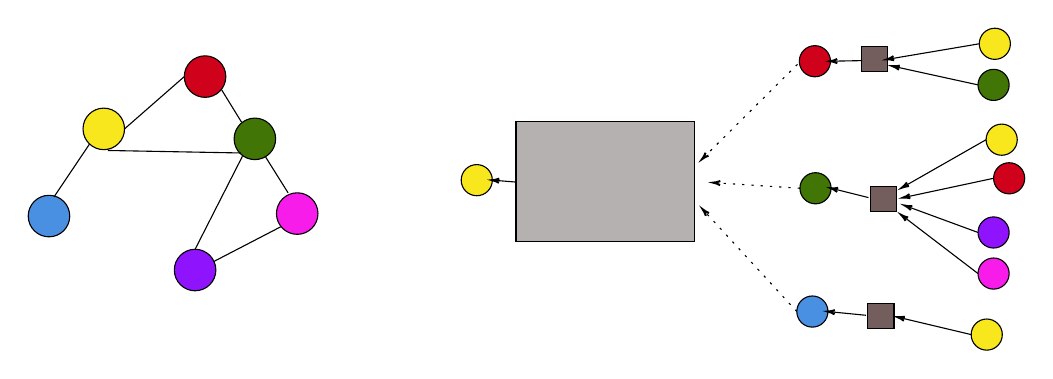
\begin{tikzpicture}[x=0.75pt,y=0.75pt,yscale=-1,xscale=1]
\tikzset{every picture/.style={line width=0.75pt}} %set default line width to 0.75pt        
\begin{scope}[scale=0.4, transform shape, shift={(0,50)}]
%Shape: Circle [id:dp7391127131517923] 
\draw  [fill={rgb, 255:red, 248; green, 231; blue, 28 }  ,fill opacity=1 ] (149,102) .. controls (149,88.19) and (160.19,77) .. (174,77) .. controls (187.81,77) and (199,88.19) .. (199,102) .. controls (199,115.81) and (187.81,127) .. (174,127) .. controls (160.19,127) and (149,115.81) .. (149,102) -- cycle ;
%Shape: Circle [id:dp5040331320120275] 
\draw  [fill={rgb, 255:red, 74; green, 144; blue, 226 }  ,fill opacity=1 ] (83,207) .. controls (83,193.19) and (94.19,182) .. (108,182) .. controls (121.81,182) and (133,193.19) .. (133,207) .. controls (133,220.81) and (121.81,232) .. (108,232) .. controls (94.19,232) and (83,220.81) .. (83,207) -- cycle ;
%Shape: Circle [id:dp45053378439553704] 
\draw  [fill={rgb, 255:red, 208; green, 2; blue, 27 }  ,fill opacity=1 ] (271,39) .. controls (271,25.19) and (282.19,14) .. (296,14) .. controls (309.81,14) and (321,25.19) .. (321,39) .. controls (321,52.81) and (309.81,64) .. (296,64) .. controls (282.19,64) and (271,52.81) .. (271,39) -- cycle ;
%Shape: Circle [id:dp8075474740173365] 
\draw  [fill={rgb, 255:red, 65; green, 117; blue, 5 }  ,fill opacity=1 ] (331,114) .. controls (331,100.19) and (342.19,89) .. (356,89) .. controls (369.81,89) and (381,100.19) .. (381,114) .. controls (381,127.81) and (369.81,139) .. (356,139) .. controls (342.19,139) and (331,127.81) .. (331,114) -- cycle ;
%Shape: Circle [id:dp8258879038376108] 
\draw  [fill={rgb, 255:red, 248; green, 28; blue, 235 }  ,fill opacity=1 ] (382,204) .. controls (382,190.19) and (393.19,179) .. (407,179) .. controls (420.81,179) and (432,190.19) .. (432,204) .. controls (432,217.81) and (420.81,229) .. (407,229) .. controls (393.19,229) and (382,217.81) .. (382,204) -- cycle ;
%Shape: Circle [id:dp23058756536424663] 
\draw  [fill={rgb, 255:red, 144; green, 19; blue, 254 }  ,fill opacity=1 ] (259,272) .. controls (259,258.19) and (270.19,247) .. (284,247) .. controls (297.81,247) and (309,258.19) .. (309,272) .. controls (309,285.81) and (297.81,297) .. (284,297) .. controls (270.19,297) and (259,285.81) .. (259,272) -- cycle ;
%Straight Lines [id:da09378991089450528] 
\draw    (157,120) -- (114,184) ;
%Straight Lines [id:da1955970352844556] 
\draw    (341,135) -- (284,247) ;
%Straight Lines [id:da49392961509251854] 
\draw    (387,220) -- (306,262) ;
%Straight Lines [id:da025955503302143468] 
\draw    (316,55) -- (340,94) ;
%Straight Lines [id:da520988735232341] 
\draw    (369,136) -- (396,179) ;
%Straight Lines [id:da03707214460650876] 
\draw    (271,39) -- (199,102) ;
%Straight Lines [id:da132312312313] 
\draw    (179,128) -- (339,131) ;
\end{scope}

%uncomment if require: \path (0,641); %set diagram left start at 0, and has height of 641
\begin{scope}[scale=0.3, transform shape, shift={(800,0)}]
%Shape: Circle [id:dp7391127131517923] 
\draw  [fill={rgb, 255:red, 248; green, 231; blue, 28 }  ,fill opacity=1 ] (6,285) .. controls (6,271.19) and (17.19,260) .. (31,260) .. controls (44.81,260) and (56,271.19) .. (56,285) .. controls (56,298.81) and (44.81,310) .. (31,310) .. controls (17.19,310) and (6,298.81) .. (6,285) -- cycle ;
%Shape: Circle [id:dp5040331320120275] 
\draw  [fill={rgb, 255:red, 74; green, 144; blue, 226 }  ,fill opacity=1 ] (545,496) .. controls (545,482.19) and (556.19,471) .. (570,471) .. controls (583.81,471) and (595,482.19) .. (595,496) .. controls (595,509.81) and (583.81,521) .. (570,521) .. controls (556.19,521) and (545,509.81) .. (545,496) -- cycle ;
%Shape: Circle [id:dp45053378439553704] 
\draw  [fill={rgb, 255:red, 208; green, 2; blue, 27 }  ,fill opacity=1 ] (549,94) .. controls (549,80.19) and (560.19,69) .. (574,69) .. controls (587.81,69) and (599,80.19) .. (599,94) .. controls (599,107.81) and (587.81,119) .. (574,119) .. controls (560.19,119) and (549,107.81) .. (549,94) -- cycle ;
%Shape: Circle [id:dp8075474740173365] 
\draw  [fill={rgb, 255:red, 65; green, 117; blue, 5 }  ,fill opacity=1 ] (550,298) .. controls (550,284.19) and (561.19,273) .. (575,273) .. controls (588.81,273) and (600,284.19) .. (600,298) .. controls (600,311.81) and (588.81,323) .. (575,323) .. controls (561.19,323) and (550,311.81) .. (550,298) -- cycle ;
%Shape: Circle [id:dp7563216956134695] 
\draw  [fill={rgb, 255:red, 248; green, 231; blue, 28 }  ,fill opacity=1 ] (838,66) .. controls (838,52.19) and (849.19,41) .. (863,41) .. controls (876.81,41) and (888,52.19) .. (888,66) .. controls (888,79.81) and (876.81,91) .. (863,91) .. controls (849.19,91) and (838,79.81) .. (838,66) -- cycle ;
%Shape: Circle [id:dp8878052396288514] 
\draw  [fill={rgb, 255:red, 65; green, 117; blue, 5 }  ,fill opacity=1 ] (836,132) .. controls (836,118.19) and (847.19,107) .. (861,107) .. controls (874.81,107) and (886,118.19) .. (886,132) .. controls (886,145.81) and (874.81,157) .. (861,157) .. controls (847.19,157) and (836,145.81) .. (836,132) -- cycle ;
%Shape: Circle [id:dp32002945113695325] 
\draw  [fill={rgb, 255:red, 248; green, 231; blue, 28 }  ,fill opacity=1 ] (849,220) .. controls (849,206.19) and (860.19,195) .. (874,195) .. controls (887.81,195) and (899,206.19) .. (899,220) .. controls (899,233.81) and (887.81,245) .. (874,245) .. controls (860.19,245) and (849,233.81) .. (849,220) -- cycle ;
%Shape: Circle [id:dp3683318015589876] 
\draw  [fill={rgb, 255:red, 248; green, 231; blue, 28 }  ,fill opacity=1 ] (825,533) .. controls (825,519.19) and (836.19,508) .. (850,508) .. controls (863.81,508) and (875,519.19) .. (875,533) .. controls (875,546.81) and (863.81,558) .. (850,558) .. controls (836.19,558) and (825,546.81) .. (825,533) -- cycle ;
%Shape: Circle [id:dp34119215740916453] 
\draw  [fill={rgb, 255:red, 208; green, 2; blue, 27 }  ,fill opacity=1 ] (861,282) .. controls (861,268.19) and (872.19,257) .. (886,257) .. controls (899.81,257) and (911,268.19) .. (911,282) .. controls (911,295.81) and (899.81,307) .. (886,307) .. controls (872.19,307) and (861,295.81) .. (861,282) -- cycle ;
%Shape: Circle [id:dp7106208118051622] 
\draw  [fill={rgb, 255:red, 144; green, 19; blue, 254 }  ,fill opacity=1 ] (836,369) .. controls (836,355.19) and (847.19,344) .. (861,344) .. controls (874.81,344) and (886,355.19) .. (886,369) .. controls (886,382.81) and (874.81,394) .. (861,394) .. controls (847.19,394) and (836,382.81) .. (836,369) -- cycle ;
%Shape: Circle [id:dp8894496983563955] 
\draw  [fill={rgb, 255:red, 248; green, 28; blue, 235 }  ,fill opacity=1 ] (836,435) .. controls (836,421.19) and (847.19,410) .. (861,410) .. controls (874.81,410) and (886,421.19) .. (886,435) .. controls (886,448.81) and (874.81,460) .. (861,460) .. controls (847.19,460) and (836,448.81) .. (836,435) -- cycle ;
%Shape: Rectangle [id:dp32031658300689125] 
\draw  [fill={rgb, 255:red, 115; green, 93; blue, 93 }  ,fill opacity=1 ] (649,71) -- (691,71) -- (691,111) -- (649,111) -- cycle ;
%Shape: Rectangle [id:dp24948896109333862] 
\draw  [fill={rgb, 255:red, 115; green, 93; blue, 93 }  ,fill opacity=1 ] (663,295) -- (705,295) -- (705,335) -- (663,335) -- cycle ;
%Shape: Rectangle [id:dp1640437735384026] 
\draw  [fill={rgb, 255:red, 115; green, 93; blue, 93 }  ,fill opacity=1 ] (659,483) -- (701,483) -- (701,523) -- (659,523) -- cycle ;
%Straight Lines [id:da9391818246381771] 
\draw    (838,66) -- (691.97,90.67) ;
\draw [shift={(690,91)}, rotate = 350.41] [color={rgb, 255:red, 0; green, 0; blue, 0 }  ][line width=0.75]    (10.93,-3.29) .. controls (6.95,-1.4) and (3.31,-0.3) .. (0,0) .. controls (3.31,0.3) and (6.95,1.4) .. (10.93,3.29)   ;
%Straight Lines [id:da565096922762111] 
\draw    (836,132) -- (700.95,102.43) ;
\draw [shift={(699,102)}, rotate = 12.35] [color={rgb, 255:red, 0; green, 0; blue, 0 }  ][line width=0.75]    (10.93,-3.29) .. controls (6.95,-1.4) and (3.31,-0.3) .. (0,0) .. controls (3.31,0.3) and (6.95,1.4) .. (10.93,3.29)   ;
%Straight Lines [id:da5786147404656463] 
\draw    (849,220) -- (715.74,296.01) ;
\draw [shift={(714,297)}, rotate = 330.3] [color={rgb, 255:red, 0; green, 0; blue, 0 }  ][line width=0.75]    (10.93,-3.29) .. controls (6.95,-1.4) and (3.31,-0.3) .. (0,0) .. controls (3.31,0.3) and (6.95,1.4) .. (10.93,3.29)   ;
%Straight Lines [id:da3777046677396121] 
\draw    (861,282) -- (717.96,312.58) ;
\draw [shift={(716,313)}, rotate = 347.93] [color={rgb, 255:red, 0; green, 0; blue, 0 }  ][line width=0.75]    (10.93,-3.29) .. controls (6.95,-1.4) and (3.31,-0.3) .. (0,0) .. controls (3.31,0.3) and (6.95,1.4) .. (10.93,3.29)   ;
%Straight Lines [id:da13099380674781425] 
\draw    (836,369) -- (720.88,326.69) ;
\draw [shift={(719,326)}, rotate = 20.18] [color={rgb, 255:red, 0; green, 0; blue, 0 }  ][line width=0.75]    (10.93,-3.29) .. controls (6.95,-1.4) and (3.31,-0.3) .. (0,0) .. controls (3.31,0.3) and (6.95,1.4) .. (10.93,3.29)   ;
%Straight Lines [id:da8218277516683541] 
\draw    (836,435) -- (714.59,342.21) ;
\draw [shift={(713,341)}, rotate = 37.39] [color={rgb, 255:red, 0; green, 0; blue, 0 }  ][line width=0.75]    (10.93,-3.29) .. controls (6.95,-1.4) and (3.31,-0.3) .. (0,0) .. controls (3.31,0.3) and (6.95,1.4) .. (10.93,3.29)   ;
%Straight Lines [id:da3800136341254434] 
\draw    (825,533) -- (708.95,505.46) ;
\draw [shift={(707,505)}, rotate = 13.35] [color={rgb, 255:red, 0; green, 0; blue, 0 }  ][line width=0.75]    (10.93,-3.29) .. controls (6.95,-1.4) and (3.31,-0.3) .. (0,0) .. controls (3.31,0.3) and (6.95,1.4) .. (10.93,3.29)   ;
%Shape: Rectangle [id:dp8336434429346229] 
\draw  [fill={rgb, 255:red, 181; green, 177; blue, 177 }  ,fill opacity=1 ] (94,191) -- (380,191) -- (380,384) -- (94,384) -- cycle ;
%Straight Lines [id:da8646710277987533] 
\draw    (650,93) -- (601,93.96) ;
\draw [shift={(599,94)}, rotate = 358.88] [color={rgb, 255:red, 0; green, 0; blue, 0 }  ][line width=0.75]    (10.93,-3.29) .. controls (6.95,-1.4) and (3.31,-0.3) .. (0,0) .. controls (3.31,0.3) and (6.95,1.4) .. (10.93,3.29)   ;
%Straight Lines [id:da47185496942409855] 
\draw    (660,313) -- (601.94,298.49) ;
\draw [shift={(600,298)}, rotate = 14.04] [color={rgb, 255:red, 0; green, 0; blue, 0 }  ][line width=0.75]    (10.93,-3.29) .. controls (6.95,-1.4) and (3.31,-0.3) .. (0,0) .. controls (3.31,0.3) and (6.95,1.4) .. (10.93,3.29)   ;
%Straight Lines [id:da9427367877844224] 
\draw    (656,502) -- (596.99,496.2) ;
\draw [shift={(595,496)}, rotate = 5.62] [color={rgb, 255:red, 0; green, 0; blue, 0 }  ][line width=0.75]    (10.93,-3.29) .. controls (6.95,-1.4) and (3.31,-0.3) .. (0,0) .. controls (3.31,0.3) and (6.95,1.4) .. (10.93,3.29)   ;
%Straight Lines [id:da6975699009927117] 
\draw  [dash pattern={on 0.84pt off 2.51pt}]  (546,99) -- (394.42,249.59) ;
\draw [shift={(393,251)}, rotate = 315.19] [color={rgb, 255:red, 0; green, 0; blue, 0 }  ][line width=0.75]    (10.93,-3.29) .. controls (6.95,-1.4) and (3.31,-0.3) .. (0,0) .. controls (3.31,0.3) and (6.95,1.4) .. (10.93,3.29)   ;
%Straight Lines [id:da05656005457935409] 
\draw  [dash pattern={on 0.84pt off 2.51pt}]  (550,298) -- (413,289.13) ;
\draw [shift={(411,289)}, rotate = 3.7] [color={rgb, 255:red, 0; green, 0; blue, 0 }  ][line width=0.75]    (10.93,-3.29) .. controls (6.95,-1.4) and (3.31,-0.3) .. (0,0) .. controls (3.31,0.3) and (6.95,1.4) .. (10.93,3.29)   ;
%Straight Lines [id:da4906087840899518] 
\draw  [dash pattern={on 0.84pt off 2.51pt}]  (545,496) -- (395.35,333.47) ;
\draw [shift={(394,332)}, rotate = 47.36] [color={rgb, 255:red, 0; green, 0; blue, 0 }  ][line width=0.75]    (10.93,-3.29) .. controls (6.95,-1.4) and (3.31,-0.3) .. (0,0) .. controls (3.31,0.3) and (6.95,1.4) .. (10.93,3.29)   ;
%Straight Lines [id:da32570331705322464] 
\draw    (93,288) -- (57.99,285.16) ;
\draw [shift={(56,285)}, rotate = 4.64] [color={rgb, 255:red, 0; green, 0; blue, 0 }  ][line width=0.75]    (10.93,-3.29) .. controls (6.95,-1.4) and (3.31,-0.3) .. (0,0) .. controls (3.31,0.3) and (6.95,1.4) .. (10.93,3.29)   ;

\end{scope}
\end{tikzpicture}
\caption{Um grafo e sua representação de adjacências para o nó amarelo em uma camada da GNN. Os blocos representam a função de agregação.}
\end{figure}
\label{fig:gnn}
\vspace{2em}

\abbrev{MLP}{\textit{multi-layer perceptron}}
A função de agregação pode ser uma soma, uma média ou a escolha dos valores
máximos e mínimos do vetor de entrada. Para que operação tenha parâmetros
treináveis, é concedido aos \textit{embeddings} adjacentes uma rede neural
multi-camadas denotada pela função MLP (do inglês \textit{multi-layer
perceptron}). O mesmo ocorre à saída da função de agregação:

\begin{equation}
    \text{AGREGA}( \{ \mathbf{h}^{(l)}_m : \forall m \in \mathcal{N}(n)\} ) = \text{MLP}_\theta\left(\sum_{m \in \mathcal{N}(n)} \text{MLP}_\phi(\mathbf{h}^{(l)}_m)\right)
\end{equation}
em que $\theta$ e $\phi$ são os parâmetros das redes MLPs,  compartilhados em
uma mesma camada $l$, e a função de agregação é a soma simples de seus
argumentos. De forma similar, a função de atualização é dada por:

\begin{equation}
    \mathbf{h}^{(l+1)}_n = \text{ATUALIZA}(\mathbf{h}^{(l)}_n, \mathbf{z}^{(l)}_n ) = f(\mathbf{W}_{\text{próprio}} \mathbf{h}^{(l)}_n + \mathbf{W}_{adj} \mathbf{z}^{(l)}_n + \mathbf{b})
\end{equation}
em que $f(\cdot)$ é uma função de ativação não-linear aplicada sobre cada
elemento do vetor, $\mathbf{W}_{\text{próprio}}$, $\mathbf{W}_{adj}$ e $\mathbf{b}$ são
as matrizes de pesos e o vetor de \textit{bias} da rede neural.

% \section{Representação dos dados}
% \subsection{\textit{One-hot encoding}}
% - Representação binária de vetores;
% - Todos os itens representados são ortogonais entre si;
% - Em conjuntos com variedade de representações, pode acarretar em alta dimensionaliade;
% \subsection{Embeddings}
% - Representação vetorial de itens;
% - Gera uma representação comprimida dos dados, com menor dimensionalidade;
% - É possível calcular a similaridade entre vetores, por ex, a partir da norma;
% - Itens não são necessariamente ortogonais;

% \section{Funções de custo}
%  Sistemas de recomendação retornam uma lista ordenada de itens candidatos
% considerando sua relevância prevista ao usuário. Esse ranqueamento pode ser
% realizado ponto a ponto, par a par ou em lista. A depender da arquitetura
% escolhida, a função de custo deve ser escolhida considerando a estabilidade

%  O ranqueamento ponto a ponto estima a pontuação ou a colocação dos itens
% independentemente uns dos outros, tal que a colocação dos itens relevantes deve
% ser baixa. O ranqueamento par a par compara a pontuação ou a colocação de pares
% de itens positivos e negativos e a função de custo impõe que a colocação do item
% positivo deve ser menor que a do negativo. O ranqueamento em lista usa as
% pontuações e as colocações de todos os itens e as compara com a ordenação
% perfeita. Como inclui ordenação, geralmente é computacionalmente mais caro e,
% portanto, não é usado com frequência. Além disso, se houver apenas um item
% relevante - como no nosso caso - o ranqueamento em lista pode ser resolvido via
% ranqueamento par a par.

% \subsection{Entropia cruzada}
% \subsection{BPR}
% \subsection{fator latente (netflix)}


% \subsection{TOP1}

% \section{Outras Técnicas}
% \subsection{Regularização}
% \subsection{Dropout}



\section{Aprendizado de Máquina aplicado ao SBRS}

As implementações de SBRS utilizam módulos, conceitos e arquiteturas
característicos dos sistemas de aprendizado de máquina. As arquiteturas de SBRS
podem ser divididas nas implementações mais simples, com abordagens básicas,
eficientes e de menor carga computacional. Essas arquiteturas são compõem a base de referência, do inglês
\textit{baseline}.

Um segundo grupo de arquiteturas de SBRS são algoritmos mais complexos e
modulares com abordagens sofisticadas de aprendizado profundo. São arquiteturas
mais intensivas computacionalmente, e que exigem uma quantidade maior de dados.
Por superarem a maioria das métricas de desempenho, algumas dessas arquiteturas
são consideradas o atual estado da arte em SBRS.

\subsection{Redes Neurais \textit{Session-Based}}
\subsubsection{CSRM}
\abbrev{CSRM}{\textit{Collaborative Session-based Recommendation Machine}}
O \textit{Collaborative Session-based Recommendation Machine} (CSRM) é um modelo
híbrido que avalia o comportamento de sessões vizinhas para melhorar a
recomendação da sessão atual \cite{collaborative2018}. O modelo é composto um
codificador de memória interna, responsável por codificar informação da sessão
vigente, um codificador de memória externa, que registra as sessões mais
recentes como sessões vizinhas em potential, e um decodificador de recomendação,
que calcula a probabilidade da próxima interação com base nas saídas dos dois
codificadores.

O codificador interno é composto por uma GRU responsável por modelar
o comportamento sequencial da sessão atual, enquanto que uma segunda GRU com
mecanismo de atenção é responsável por codificar cada item de forma individual.
A saída dessas duas unidades compõem um vetor de saída para o codificador interno.

O codificador externo é uma matriz que registra as sessões mais recentes em
ordem cronológica. Em seguida, é calculada a similaridade de cada uma em relação
à sessão vigente. As maiores similaridades são selecionadas e utilizadas para
calcular os pesos que compõem o vetor de saída do codificador.

O decodificador de recomendação recebe os vetores de saída dos dois
codificadores para calcular a probabilidade de um item candidato ser o próximo
item em determinada sessão. Para maximizar a probabilidade de predição de um
item que de fato foi selecionado, a função de custo por entropia cruzada é
empregada.

\subsubsection{GRU4Rec}
GRU4Rec  \cite{gru4rec_1, gru4rec_2} é uma RNN com unidades GRU modificadas, as
quais são treinadas em \textit{mini-batches}, ou seja, em pequenas bateladas de
amostras de treinamento. Essa forma de treinamento aproveita a capacidade de
paralelismo do \textit{hardware} e da própria arquitetura do modelo, tornando a
convergência do gradiente descendente mais rápida e estável.

Na saída, a rede calcula as pontuações apenas para os itens marcados como
alvo do treinamento supervisionado, uma vez que o cálculo das
pontuações para todos os itens de uma base esparsa seria inviável. Essa amostra
na saída é marcada com pontuação máxima quando o item de fato está presente, e
negativa quando o alvo de outra sessão é amostrado. A ideia é que itens
populares os quais o usuário não interagiu são de conhecimento dele, mas sem
interesse, o que deve ser reforçado com uma pontuação negativa.

\abbrev{BPR}{Ranqueamento Bayesiano Personalizado}
A função de custo, que pertence ao grupo de funções \textit{learning-to-rank},
retorna o ranqueamento, isto é, a classificação ordenada dos itens de acordo com
a probabilidade de serem selecionados. É utilizado o Ranqueamento Bayesiano
Personalizado (BPR \cite{rendle2009}, do inglês \textit{Bayesian Personalized
Ranking}), com modificações visando resolver o problema de desaparecimento do
gradiente, que pode ocorrer em arquiteturas de RNNs.

\subsubsection{NextItNet}
Modela a probabilidade condicional de uma sequência de itens a partir de uma
CNN, cuja arquitetura é modificada para receber sequências de itens
\cite{nextitnet}. Essas probabilidades são obtidas a partir de uma pilha de
redes convolucionais de uma única dimensão.

A modelagem é distinta do modelo GRU4Rec, no qual modela-se na saída uma única
pdf condicional $p(x_i|x_{0:i-1}, \mathbf{\theta})$ alusiva ao último item $i$,
dado um vetor de interações entrada e os hiperparâmetros. Por sua vez, o
NextItNet modela uma pdf condicional para cada item da sequência $x_{0:i}$. Por
exemplo, para uma sequência de $[x_0, x_1, ..., x_i]$ itens, a saída prevê os
itens $[x_1, x_2, ..., x_i, x_{i+1}]$. Essa abordagem permite aplicar técnicas
de \textit{data augmentation} \cite{tan2016improved}, gerando novas amostras de
treinamento a partir de amostras existentes.

O modelo utiliza convolução dilatada: uma técnica que aumenta o tamanho do
núcleo ao preenchê-lo com zeros nos espaços entre os valores existentes. Dessa
forma, o campo receptivo da rede aumenta para uma mesma quantidade de
parâmetros. No modelo em questão, sessões com uma grande quantidade de
interações conseguem ser modeladas com menos parâmetros, aumentando a eficiência
do modelo.

A arquitetura da NextItNet utiliza blocos residuais, proporcionando vantagens em
comparação às CNNs tradicionais \cite{he2016deep}. Um aspecto das CNNs
tradicionais durante o treinamento é o acúmulo de ruído nos valores produzidos
pela camada de saída. Isso ocorre devido aos pesos aleatórios na inicialização
da rede, resultando em uma convergência lenta do gradiente em redes profundas.

Os blocos residuais tratam dessa questão ao agrupar as camadas da rede em
blocos, tal que a entrada de cada bloco é diretamente transmitida à entrada do
bloco seguinte, somada ou concatenada à saída do bloco anterior. Isso elimina a
necessidade de os blocos aprenderem quais informações da camada de entrada devem
ser selecionadas ou transmitidas, já que essa informação é passada diretamente
pela entrada.

Outra característica importante dos blocos residuais é o gradiente
calculado pela função de custo ser transmitido para cada bloco residual, em vez
de ser transmitido apenas para a camada de entrada. Esse método acelera a
convergência do gradiente, proporcionando um treinamento mais eficiente e rápido
da rede.
\abbrev{PDF}{função de densidade de probabilidade}

Cada bloco residual é composto em ordem por uma camada de convolução dilatada,
uma camada de normalização, uma função de ativação ReLU, uma segunda camada de
convolução dilatada e uma segunda camada de normalização.

Outro aspecto importante da arquitetura é evitar que o item a ser previsto tenha
acesso aos itens seguintes da sequência. Isso é feito a partir de uma máscara
aplicada na entrada da rede, que realiza operações de translação e deslocamento
no vetor unidimensional de entrada.

\subsubsection{NARM}
\abbrev{NARM}{\textit{Neural Attentive Session-based Recommendation Model}}
O modelo \textit{Neural Attentive Session-based Recommendation Model} (NARM)
\cite{narm} consiste em um par codificador-decodificador com um gerador
intermediário de parâmetros entre ambos, que recebe a representação oculta do
codificador e um sinal de atenção, calculado a partir da representação oculta do
próprio codificador.

O codificador consiste em dois módulos paralelos. Ambos consistem em uma RNN de
unidades GRU. O primeiro módulo, representando um recomendador global, emite o
estado oculto apenas da última unidade GRU, visando codificar as informações do
comportamento sequencial do usuário. O segundo módulo, representando um
recomendador local, emite os estados ocultos de todas as suas unidades, visando
codificar o objetivo principal naquela sessão. Dessa forma, uma sequência de
interações do usuário que faça sentido entre si, mas que não seja relevante para
o objetivo principal, é modelada separadamente.

O sinal de atenção recebe os estados ocultos do recomendador local e global, e
calcula a similaridade entre eles. Para um item arbitrário do recomendador local, que envia os estados ocultos de
todos os itens, o sinal de atenção modela o quão importante aquele determinado
item é para o objetivo principal da sessão. Esse valor controla o quanto daquele
estado será transmitido ao decodificador. A formação do vetor intermediário de
parâmetros é realizada ao combinar os estados ocultos com seus respectivos
sinais de atenção.

Em geral, o decodificador em uma RNN utiliza uma camada completamente conectada,
o que acarreta em uma grande quantidade de parâmetros a serem alocados, tornando
o treinamento lento. Esse procedimento equivale a alocar os estados para $H$
itens da sessão e $N$ candidatos para cada predição, gerando uma matriz de
dimensões ${H \times N}$. No modelo NARM, utilizam-se $D$ \textit{embeddings} de
itens, tal que $D < N$. Um \textit{embedding} é uma representação de um espaço
vetorial de dimensões reduzidas, que comprime um espaço vetorial de dimensões
maiores.

Em seguida, uma camada é responsável por calcular a
similaridade entre os parâmetros intermediários e os \textit{embeddings} dos
itens, cujo resultado é emitido a uma camada de função \textit{softmax}, obtendo
a probabilidade de cada item ser o próximo da sessão. O modelo é treinado em \textit{mini-batches}, tal qual o modelo GRU4REC. A
função de custo é a entropia cruzada.


\subsubsection{SR-GNN}
\abbrev{SR-GNN}{\textit{Session-based Recommendation with Graph Neural Networks}}
O modelo \textit{Session-based Recommendation with Graph Neural Networks}
(SR-GNN) utiliza uma rede neural em grafos com unidades GRU e mecanismo de
atenção, representando internamente os dados como \textit{embeddings} de itens
e \textit{embeddings} de sessões. \cite{gnn}.

Na bibliografia descritiva do modelo, os autores identificam dois problemas
comuns das demais arquiteturas. O primeiro é a dificuldade em prever
corretamente qual o usuário associado à sessão prevista, uma vez que em muitas
bases de dados e situações reais, o usuário é anônimo, ao contrário da abordagem
\textit{session-aware}. O segundo problema é a modelagem da sessão em transições
de itens consecutivos em um único caminho, negligenciando transições entre
contextos distintos que acarretam em itens distintos na sessão. Por
consequência, transições mais complexas são negligenciadas por esses modelos
\textit{session-based}. Por esses motivos, os autores optaram por dispensar a
modelagem de usuários e optaram por uma GNN.

% Each session sequence s can be modeled as a directed graph Gs = (Vs,Es). In this session graph, each node represents an item vs,i ∈ V . Each edge (vs,i−1, vs,i) ∈ Es means that a user clicks item vs,i after vs,i−1 in the session s. Since sev- eral items may appear in the sequence repeatedly, we assign each edge with a normalized weighted, which is calculated as the occurrence of the edge divided by the outdegree of that edge’s start node. We embed every item v ∈ V into an unified embedding space and the node vector v ∈ Rd indicates the latent vector of item v learned via graph neu- ral networks, where d is the dimensionality. Based on node vectors, each session s can be represented by an embedding vector s, which is composed of node vectors used in that graph.
Inicialmente, cada sessão é modelada como um grafo orientado, com arestas
direcionadas ao item subsequente, tal que demais sessões que tenham os mesmos
itens também são incluídas no mesmo grafo. Cada grafo é representado por uma
matriz de adjacências modificada, dada a necessidade de representar a ordem das
transições. Por sua vez, a GNN recebe essa matriz e gera um vetor de
\textit{embeddings} para os itens daquela sessão, capturando e extraindo suas
características representativas. Uma característica importante dessa GNN é a inclusão
de portas de \textit{reset} e \textit{update}, controlando quais informações
serão preservadas ou descartadas.

A partir dos \textit{embeddings} de itens, são gerados dois \textit{embeddings}
de sessões. O primeiro é chamado de \textit{embedding} local, composto por um
vetor simples $s = [v_{s,1}, v_{s,2}, \ldots, v_{s,n}],$ no qual $v_{s,i}$ é o
\textit{embedding} do i-ésimo item da sessão $s$. O segundo é chamado de
\textit{embedding} global, gerado a partir de um mecanismo de atenção, na
abordagem de atenção suave (do inglês \textit{soft-attention}). A partir dessas
duas representações, gera-se um \textit{embedding} híbrido ao concatenar os dois
vetores e comprimi-los em uma única matriz com representação matricial de menor
dimensão.

O \textit{embedding} híbrido é utilizado para calcular a probabilidade do próximo item
da sessão. Para isso, é utilizada uma função de ativação \textit{softmax}. A função de custo
empregada é a entropia cruzada.

\subsubsection{STAMP}
\abbrev{STAMP}{\textit{Short-Term Attention/Memory Priority}}
O modelo \textit{Short-Term Attention/Memory Priority} (STAMP)~\cite{stamp}, assim como o
modelo NARM, distingue e identifica os padrões de curto e longo prazo
nas interações dos usuários. Sua principal diferença é o reforço explícito na
última interação realizada na sessão, como medida para realizar essa distinção.

Um ponto levantado pelos autores a modelos baseados em filtragem colaborativa,
fatoração de matrizes e cadeias de Markov é a dificuldade em adaptarem-se para
padrões de curto prazo, favorecendo padrões de preferência geral. Por outro
lado, modelos baseados em aprendizado profundo são capazes de, em sua modelagem,
lidarem com esse tipo de problema. No caso particular do STAMP, a ênfase
explícita na última interação da sessão permite que o modelo extraia atributos
tanto do objetivo principal da sessão quanto de desvios de curto prazo nela.

Primeiramente, o modelo gera um vetor de \textit{embeddings} para cada item da
sessão. O próprio modelo deve aprender a gerar a representação em
\textit{embedding} para cada item.

O mecanismo de atenção escolhido é uma rede neural \textit{feed-forward}, em que
o coeficiente de atenção para o i-ésimo item é calculado com uma função de
ativação sigmoide. A função recebe uma combinação linear dos \textit{embeddings} do
i-ésimo item, do último item da sessão e da motivação geral da sessão. A
motivação geral da sessão é calculada como uma média ponderada dos
\textit{embeddings} de todos os itens exceto o mais recente, cujos pesos
equivalem a um decaimento: quanto mais recente o item, mais decai o peso.

Ao obter os coeficientes de atenção, o interesse geral baseado em atenção é
calculado como a média ponderada dos \textit{embeddings} dos itens, cujos pesos
são os coeficientes de atenção. Enquanto o interesse geral é representado por
esse vetor, o interesse momentâneo é dado pelo \textit{embedding} do último item
da sessão. 

\subsection{Redes Neurais \textit{Session-Aware}}

\subsubsection{HGru4Rec}

O modelo HGru4Rec propõe o uso de uma RNN hierárquica, ou HRNN, para
recomendação \textit{session-based}. Na HRNN, o estado oculto de uma RNN de
baixo-nível é repassado à entrada de uma RNN de alto-nível. A RNN de alto-nível
é responsável por prever um vetor de inicialização para o próximo estado da RNN
de baixo-nível. Os estados ocultos dessas redes são compostas por GRUs.

No caso do HGru4Rec, cada unidade é composta por duas GRUs. A primeira GRU, à
nível de sessão, é responsável por modelar a atividade do usuário dentro de
sessões e gerar recomendações. A segunda GRU, à nível de usuário, é responsável
por modelar a evolução das preferências dos usuários entre as sessões, além de
inicializar a GRU da próxima sessão. A modelagem de usuário faz com que essa abordagem
seja \textit{session-aware}.

% explicar que usa mini-batch training
O modelo é treinado em \textit{mini-batches}. A função de custo utilizada foi a
  TOP1 \cite{HidasiKBT15}, que consiste na posição relativa do item relevante,
  calculada como:
  \begin{equation}
    L_s = \frac{1}{N_s} \sum_{j=1}^{N_s}I\{ \hat{r}_{s,j} > \hat{r}_{s,i}\}
  \end{equation}
  em que $N_s$ é o tamanho da amostra, $I$ é a função indicadora aproximada por
  uma sigmoide, $i$ é o item em questão da predição e $j$ é um item da amostra.

\subsubsection{IIRNN}
\abbrev{IIRNN}{\textit{Inter-Intra Recurrent Neural Network}}
  O principal objetivo do modelo IIRNN~\cite{skrede2017inter} (Inter-Intra RNN) é aumentar a acurácia
ao prever os itens iniciais de uma sessão. Em geral, as preferências da sessão
vigente no início de uma sessão em uma situação de \textit{cold-start} não são
suficientes para recomendar de forma acurada, seja pela falta de contexto
daquela própria sessão ou pela falta de um histórico recente do usuário. O
modelo IIRNN trata desse problema com o uso de uma RNN intra-sessões e uma RNN
inter-sessões.

A RNN intra-sessões é responsável por modelar o comportamento do usuário dentro
da sessão vigente, de forma similar a outros modelos com RNNs
\cite{HidasiKBT15}. O \textit{embedding} dos itens e o estado oculto na saída da
RNN inter-sessões são utilizados como entradas para uma ou mais camadas de GRUs,
que por sua vez geram estados ocultos. Essa RNN utiliza o mecanismo de
\textit{dropout}, que consiste em desativar aleatoriamente algumas unidades da
rede durante o treinamento. Dessa forma, a rede generaliza melhor os dados de
entrada e evita o \textit{overfitting}. Os estados ocultos são emitidos a uma camada
\textit{feed-forward}, responsável por gerar a predição.

Existem duas formar de treinar a RNN inter-sessões: a partir do
\textit{embedding} imediatamente anterior ao item atual na sessão, ou a partir
da média dos vetores de \textit{embedding} de todos os itens da sessão. Esse
segundo método chama-se \textit{average pooling}. A depender da aplicação ou do
conjunto de dados, uma das duas formas apresenta melhores resultados.

Durante o treinamento em \textit{mini-batches}, os itens mais recentes das
sessões são reservados ao conjunto de teste. Além disso, sessões de um mesmo
usuário são ordenadas temporalmente em uma mesma batelada, tal que as
sessões mais recentes são processadas por último. Por fim, cada batelada
deve conter uma variedade de usuários, sem representar desproporcionalmente
determinado usuário. Essas medidas são tomadas propositalmente para enviesar o
modelo às preferências mais recentes dos usuários, mantendo capacidade de
generalização. 

\subsubsection{NCSF}
\abbrev{NCSF}{\textit{Neural Cross-Session Filtering}}
Os autores do modelo \textit{Neural Cross-Session Filtering} (NCSF)~\cite{hu2018neural} discorrem
sobre três problemas que afetam o desempenho em sistemas de recomendação
\textit{session-based}: a falta do contexto da sessão, em que um item adquirido
recentemente pode significar a falta de desejo nele; a modelagem da ordem dos
itens de forma rígida, em situações em que a ordem não é determinante; e a
distinção entre os contextos intra e inter-sessão, tal como o modelo IIRNN aborda.
Dessa forma, o modelo NCSF propõe o uso de um codificador associado ao histórico de sessões
e outro associado à sessão vigente. Um terceiro codificador recebe os estados ocultos das saídas
dos dois primeiros codificadores e gera a predição.

O codificador de histórico de sessões consiste em RNN de camadas GRU. O
codificador recebe como entrada \textit{embeddings} de sessões. Esses
\textit{embeddings} são gerados a partir dos \textit{embeddings} de itens
ponderados cada um por um peso, representando o quão relevante determinado item
é dentro do contexto da sessão vigente, independente da ordem ou da proximidade
na sequência de itens. Esse peso é calculado por um mecanismo de atenção com uma
rede neural de duas camadas. O estado oculto da sessão anterior à sessão vigente
é emitido na saída.

O codificador da sessão vigente também recebe o \textit{embedding} de sessão
gerado por mecanismo de atenção. Nesse caso, o estado oculto na saída é função
tangente hiperbólica aplicada sobre o \textit{embedding} mencionado. Em seguida,
as saídas dos dois codificadores são repassadas a um codificador intra e
inter-sessão. Uma função de ativação é utilizada como porta, filtrando a
informação dos dois codificadores anteriores. Essa função concatena os dois
vetores de saída, aplicando um peso e uma função sigmoide em seguida, gerando o
vetor de porta. A partir desse vetor, o veto de \textit{embedding} do contexto
é calculado como a combinação linear dos dois \textit{embeddings} de sessão,
ponderados pelo vetor de porta.

Finalmente, a pontuação associada ao item-alvo e sua probabilidade condicional
dado o vetor de contexto são calculados a partir de uma função softmax.
  
\subsubsection{NSAR}
\abbrev{NSAR}{\textit{Neural Session-Aware Recommender}} O modelo \textit{Neural
Session-Aware Recommender} (NSAR)~\cite{phuong2019neural} é uma RNN de camadas
GRU, com a representação do usuário inserida no modelo, de forma análoga à
representação dos itens e sessões. Dessa forma, o \textit{embedding} de usuário
é combinado ao estado oculto na saída de cada GRU.

A combinação entre os \textit{embeddings} de usuário e de sessão ocorre de forma
adaptativa, alternando a importância entre a sequência de itens ou o usuário
representado. Para isso, é modelado um mecanismo de portas. Para calcular um
peso que será associado a cada um dos \textit{embeddings}, os
\textit{embeddings} de usuário e de sessão sofrem uma sequência de operações em
funções de ativação. É calculada a similaridade dos \textit{embeddings} por um
vetor de contexto de usuário e outro de sessão. Dessa forma, é possível
identificar e abstrair quais usuários possuem preferências consistentes entre
sessões e quais itens influenciam fortemente os eventos subsequentes. Os pesos
obtidos ao final desse processo ponderam a combinação linear entre os dois
\textit{embeddings}, tal que esse resultado é aplicado a uma função softmax,
gerando a probabilidade do item subsequente.

\subsubsection{SHAN}
\abbrev{SHAN}{\textit{Sequential Hierarchical Attention Network}}
A arquitetura \textit{Sequential Hierarchical Attention Network} (SHAN) utiliza uma rede
de atenção hierárquica, capturando preferências de longo prazo a partir de um
mecanismo de atenção, as quais são combinadas com os interesses de curto
prazo~\cite{shan}.

Primeiramente, as sessões anteriores à sessão vigente compõem o conjunto de
sessões de longo prazo. Uma primeira rede neural atua como mecanismo de atenção
sobre esse conjunto de sessões. Para isso, os \textit{embeddings} dos itens
dessas sessões e o \textit{embedding} usuário associado a essas sessões são
utilizados como entrada. As funções de ativação calculam a pontuação de atenção
para cada item. É realizado o \textit{pooling} de atenção, ponderando e somando
os \textit{embeddings} dos itens de acordo com suas pontuações, o que gera um
vetor representativo das preferências de longo prazo.

De forma similar à primeira etapa, uma segunda rede neural atua como mecanismo
de atenção sobre a sessão vigente. Nesse caso, o \textit{embedding} do usuário associado
às sessões, os \textit{embeddings} dos itens da sessão vigente e o vetor de
preferências de longo prazo são utilizados como entrada. Ao final do \textit{pooling}
de atenção para essa segunda etapa, é gerado um vetor híbrido, que combina
preferências de longo e curto prazo.

Uma matriz representativa da preferência do usuário para um item candidato é
dado pelo produto do \textit{embedding} desse item com o vetor híbrido, de forma
análoga a um modelo de fator latente. Por fim, essa matriz e os demais
parâmetros do modelo são utilizados para treinar um modelo de máxima
probabilidade a posteriori.

\subsection{Métodos Baseados em Fatoração}

\subsubsection{FPMC}
\abbrev{FPMC}{\textit{Factorized Personalized Markov Chains}} O modelo
\textit{Factorized Personalized Markov Chains} (FPMC) é um modelo que utiliza
cadeias de Markov para recomendações de cestas de itens~\cite{mkv}.

Uma cadeia de Markov de ordem $m$ é definida como a probabilidade condicional de
um evento dados os $m$ eventos anteriores. Visando simplificar o modelo, o
modelo FPMC utiliza uma cadeia de Markov de ordem $1$, ou seja, a probabilidade
condicional de um evento dado o evento anterior. Dessa forma, a matriz de
transição do espaço de estados é suficiente para descrever a cadeia.

Uma vez que deseja-se recomendar cestas de itens, as transições entre estados
consistem em transições de valores binários representando cada item que descreve
determinada cesta. Para modelar as preferências de um único usuário, basta que a
matriz de transição tenha dimensões $|I| \times |I|$, onde $|I|$ é a quantidade
de itens distintos no conjunto de dados. Para modelar as preferências de todos
os usuários, é necessário compor um tensor de dimensão $|U| \times |I| \times
|I|$. Dessa forma, o modelo FPMC original é um modelo \textit{session-aware},
porém adaptado para recomendação \textit{session-based} no comparativo.

Uma vez que o tensor de transição seria esparso, a convergência de um modelo de
máxima verossimilhança seria inviável. Dessa forma, o modelo FPMC utiliza a
decomposição de Tucker para reduzir a dimensionalidade do tensor de transição. A
decomposição de Tucker é uma generalização da decomposição SVD para tensores ou
representações de ordem superior. A decomposição de Tucker consiste em decompor
um tensor em um núcleo e em matrizes de projeção para cada dimensão do tensor.

Ao aplicar o modelo FPMC para a tarefa de recomendação de itens, os parâmetros
do modelo são otimizados para a tarefa de ranqueamento de itens. Para isso, os
autores utilizam e adaptam o critério de otimização utilizado no modelo BPR
\cite{rendle2009}.

\subsubsection{FISM}
\abbrev{FISM}{\textit{Factorized Item Similarity Models}} O modelo
\textit{Factorized Item Similarity Models} (FISM) \cite{kabbur2013fism} é um
modelo que gera recomendações a partir da similaridade entre itens, estimados a
partir de representações em matrizes de fator latente. O modelo FISM original
não foi proposto como um modelo \textit{session-based}: Os itens avaliados por
um usuário não tem distinção de sessão, contexto ou instante de tempo, uma vez
que a fatoração de matrizes por fatores latentes não modela essas
características. Esse modelo é adaptado para o comparativo
para atuar como um modelo \textit{session-based}.

O modelo FISM gera as matrizes de vetores e fatores latentes a partir da matriz
de avaliações. Em vez de estimar uma avaliação particular como o produto entre
dois vetores das matrizes obtidas na fatoração, tal como descrito na equação
\ref{fator_latente}, o modelo FISM estima a avaliação como o somatório das
similaridades entre cada item avaliado pelo usuário e o item estimado. Essa
similaridade é obtida ao realizar o produto interno do vetor latente de cada
item avaliado com o fator latente do item a ser estimado.

\subsubsection{Fossil}
\abbrev{Fossil}{\textit{Factorized Sequential Prediction with Item Similarity Models}}
O modelo \textit{Factorized Sequential Prediction with Item Similarity Models}
(Fossil) \cite{fossil} une a abordagem baseada em similaridade do modelo FISM com a abordagem
\textit{session-aware} baseada em cadeias de Markov do modelo FPMC. O objetivo é
aproveitar a capacidade de modelar características temporais do modelo FPMC, em
razão do uso de cadeias de Markov, com a compressão sobre matrizes esparsas do
modelo FISM. Dessa forma, as preferências de longo prazo são obtidas por um
modelo de fatores latentes sobre a base completa de itens, enquanto que as
preferências de curto prazo e seus padrões sequenciais são obtidos por uma
cadeia de Markov.

\subsubsection{SMF}
\abbrev{SMF}{\textit{Session-based Matrix Factorization}} O modelo
\textit{Session-based Matrix Factorization} (SMF) \cite{ludewig_2018}
assimila-se ao modelo Fossil, ao combinar fatoração de matrizes com cadeias de
Markov. A diferença consiste na substituição da parcela responsável por modelar
as preferências de longo prazo do usuário por preferências de sessão. Essa
mudança se dá com o objetivo de tornar o modelo aplicável em situações de
\textit{cold-start}, sem necessidade de histórico de interações do usuário.

Uma fato importante sobre o comparativo entre os modelos baseados em fatoração é
o fato de os modelos originais FISM, Fossil e FPMC utilizarem
\textit{embeddings} de usuários e serem projetados para prever a próxima ação de
usuários. Não foram originalmente projetados para cenários de recomendação
\textit{session-based} com usuários anônimos. Dessa forma, a aplicação desses
modelos em cenários \textit{session-based} são adaptações de seus usos
originais~\cite{ludewig2020advances}. O único modelo originalmente projetado
para cenários \textit{session-based} é justamente o SMF.

\section{Indaband}

O aplicativo móvel Indaband contém uma série de funcionalidades e abstrações
para a gravação e distribuição de música colaborativa. Para maior entendimento
do do sistema de recomendação a ser proposto, é necessário compreender as
principais entidades do aplicativo.

\subsubsection{Sessão}

A sessão é o ambiente digital colaborativo que permite a adição, edição, remoção e mixagem de faixas. Sessão também é o nome dado ao conjunto de faixas introduzidas pelos usuários que constituem uma determinada música.

O usuário que cria a sessão é considerado seu dono. Os demais
usuários que aceitam o convite para ingressar na sessão são considerados
participantes.

A sessão contém uma funcionalidade de cabine de gravação, permitindo que os
participantes gravem faixas de áudio ou de vídeo. Além disso, o usuário pode
importar mídias de áudio ou de vídeo, tal que cada mídia importada equivale a
uma faixa.

Toda sessão publicada é disponível para visualização pública e contém ao menos
uma faixa. A publicação pode ser posteriormente removida pelo dono da sessão.


\begin{figure}[h]
  \begin{center}
    \subfigure[]{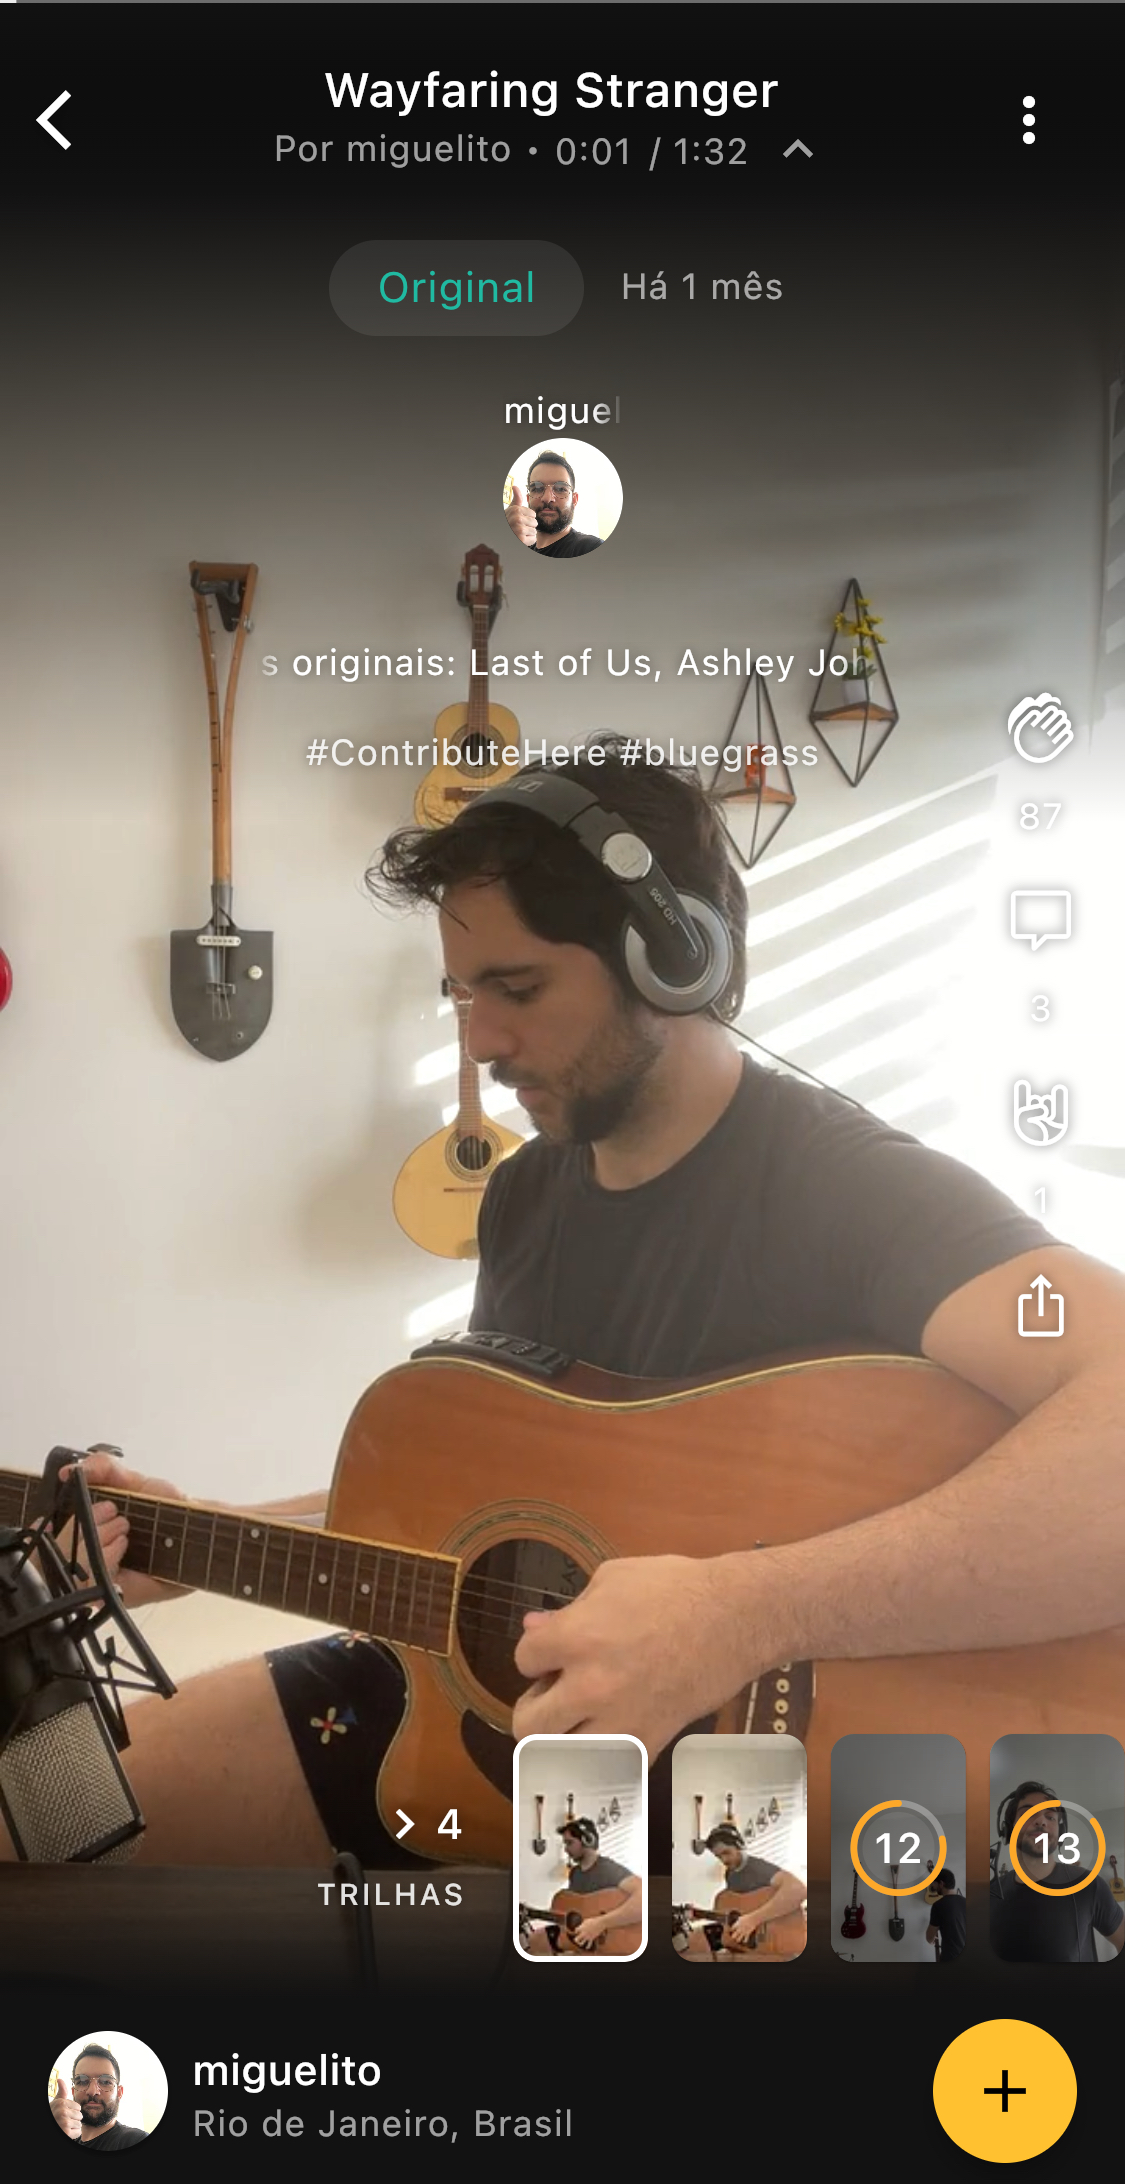
\includegraphics[width=0.4\textwidth]{chapters/chap02/images/wayfaring_original.jpeg}}
    \subfigure[]{
\includegraphics[width=0.4\textwidth]{chapters/chap02/images/wayfaring_fork.jpg}}
    \caption{Duas sessões publicadas no aplicativo Indaband. A primeira sessão é
    a sessão original, enquanto a segunda é um \textit{fork} subsequente da
    primeira. Ambas compartilham o mesmo nome e as faixas da primeira sessão. A
    segunda sessão contém faixas adicionais.}
    \label{fig:session_and_fork}
  \end{center}
  \end{figure}

\subsubsection{\textit{Fork}}
Toda sessão publicada disponibiliza a funcionalidade de \textit{fork} para os
demais usuários da plataforma. O \textit{fork} é uma cópia da sessão original,
em que é possível adicionar gravações inéditas, editar e remover faixas pré-existentes sem afetar a publicação original.

Quando publicada, a sessão \textit{fork} exibe o autor original das faixas
pré-existentes que forem mantidas, além da referência para a sessão anterior.

O \textit{fork} é uma das principais formas de colaboração assíncrona entre
usuários. A figura \ref{fig:session_and_fork} ilustra duas sessões, sendo a
segunda um \textit{fork} subseqeuente da primeira. Note que a quantidade de
faixas e usuários presentes na segunda sessão aumenta. Além disso, conta com
maior quantidade de visualizações, comentários e outras formas de engajamento
positivo. Entre essas duas sessões, houve uma série de \textit{forks}
intermediários, realizados por cada um dos usuários que adicionaram faixas às
suas sessões.


\subsubsection{Faixa}
A faixa é uma mídia com áudio e vídeo que geralmente contém a gravação de um
instrumento ou voz. Uma faixa necessariamente é criada a partir de um entre três
recursos: tal como uma gravação original, tal como um \textit{fork} de uma faixa
publicada anteriormente ou como uma importação de uma mídia de áudio ou de
vídeo.

  % \subsection{Exemplos}

  % Dois exemplos de aplicações de SBRS
  % são a recomendação de músicas em uma sessão de execução \cite{music_2013} e
  % produtos a serem adicionados em um carrinho de compras virtual
  % \cite{shopping_cart_2023}.

% \subsection{Bases de comparação não-personalizadas}

% \subsection{Bases de comparação por extração de padrões}